% The title (the club, no speaker), the hook and the challenge
\stepcounter{dcpskipped}% no footer, not counted (see preamble)
\begin{frame}
  \thispagestyle{talknofooter}
  \begin{center}
    {\huge We Have a Challenge for You!\par}
    \medskip
    {\Large A verified relational algebra library in Lean, by hand\par}
    \smallskip
    {\large (Ask us more)\par}
    \vspace{5mm}
    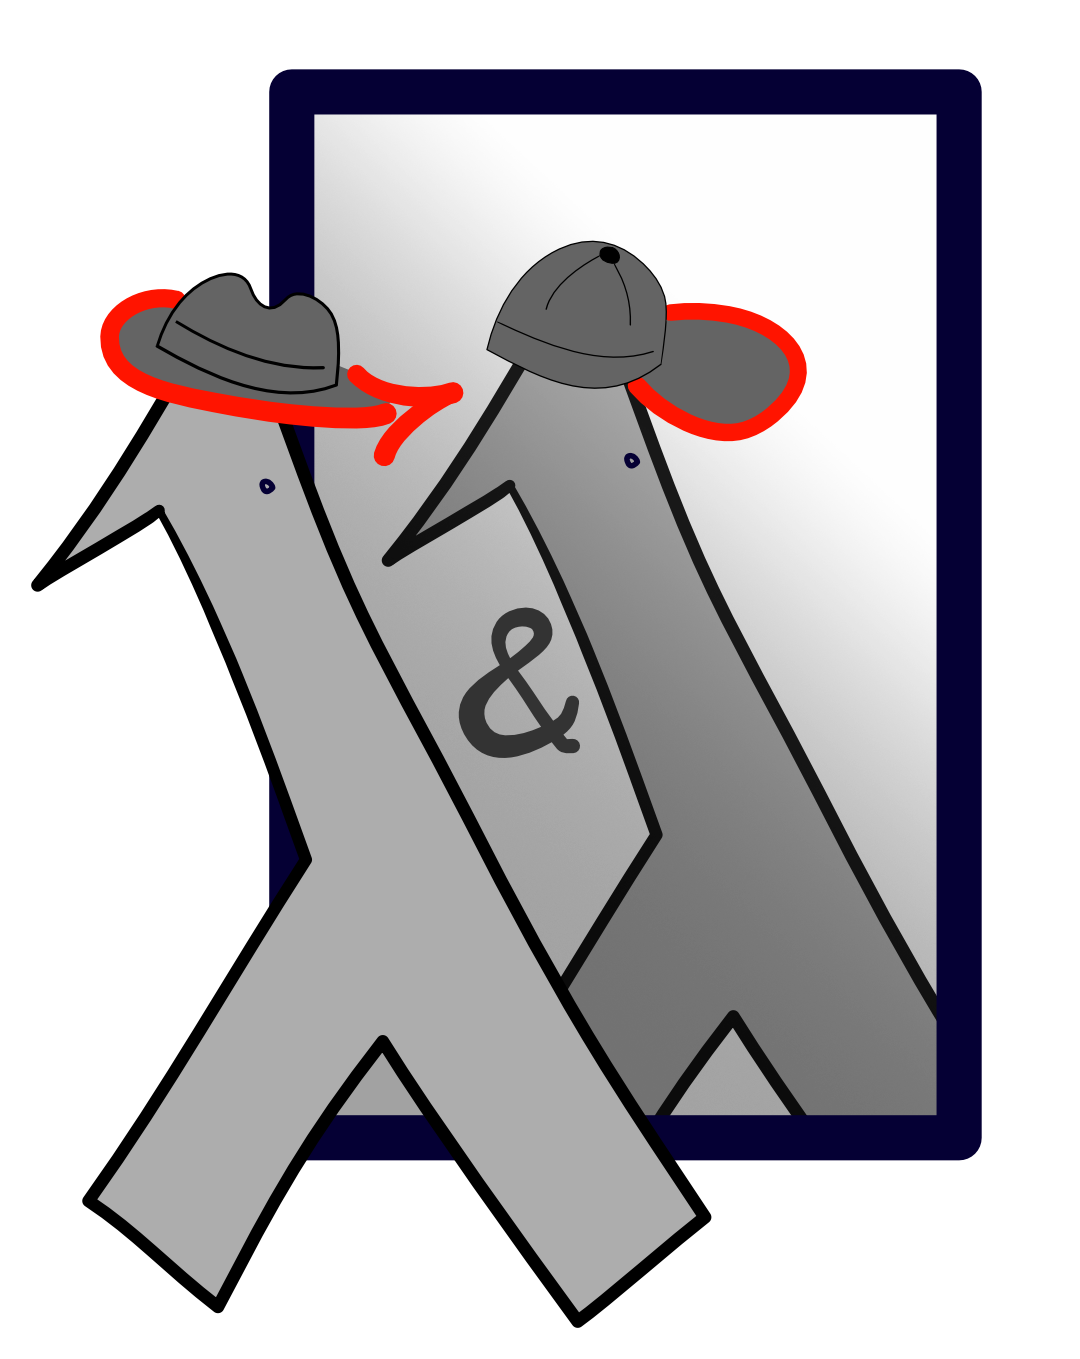
\includegraphics[height = 26mm, alt = {The Proofs and Programs Club
      logo: a lambda in a hat and its reflection in a mirror, wearing a
      different hat, with an ampersand between them}]{papc-logo.png}\par
    \medskip
    {\large The Proofs and Programs Club @ RHUL\par}
    {\small\url{https://papc-rhul.github.io/}\par}
  \end{center}
  \vfill
  {\small 19 November 2026\hfill
    
\includegraphics[height = 8mm, alt = {Royal Holloway, University of
      London logo}]{RHULLogo.png}\par}
\end{frame}

\begin{frame*}
  \frametitle{Databases Rewrite Your Queries Using Laws}
  \mainblock{sql-pushdown.sql}
  \begin{itemize}
    \item Faster, and correct only because the filter mentions nothing but
      \code{users}: a \textbf{side condition}.
    \item Get a side condition wrong and the database silently answers
      wrongly. Testing tools such as SQLancer have found hundreds of bugs in
      mature database systems.
  \end{itemize}
  \begin{sticky}[halign = center]
    Each rewrite is a \textbf{law} of relational algebra, and laws can be
    \textbf{proved}, side conditions included.
  \end{sticky}
  \slideref{SQLancer: \url{https://github.com/sqlancer/sqlancer} \rfsep
    M. Rigger, Z. Su. \textbf{Detecting Optimization Bugs in Database Engines via Non-Optimizing Reference Engine Construction}. ESEC/FSE 2020.}
\end{frame*}

\begin{frame}
  \frametitle{The Challenge: Build the Algebra, Prove Its Laws}
  \begin{sticky}[halign = center]
    Build, in \textbf{Lean}, a library for \textbf{relational algebra},
    and prove it correct. \textbf{By hand.}
  \end{sticky}
  \medskip
  {\centering\renewcommand\arraystretch{1.3}
    {\headerrow\begin{tabular}{@{}l@{\qquad}>{\raggedright\arraybackslash}p{58mm}@{\qquad}>{\raggedright\arraybackslash}p{58mm}@{}}
      \hline
      \textbf{Level} & \textbf{Build} & \textbf{Prove} \\ \hline
      1 Tables & schemas, rows, relations & (get the definitions right) \\
      2 Queries & a query language and its evaluator & bad queries cannot
        be written \\
      3 Laws & & the laws optimisers use, with their side conditions \\
      4 Optimiser & a function from queries to queries & it never changes
        an answer \\
      5 Fast joins & hash join, sort-merge join & each computes exactly the
        join \\ \hline
      Stretch & bags, NULL, aggregation, SQL & which laws survive \\
      \hline
    \end{tabular}}\par}
  \medskip
  You cannot do all of this yet: each level teaches you what the next one
  needs.
\end{frame}
